\scanpage{4}
\mspage{3}
\unsure{Stronger|Stronger} condition : \deleted{\unsure{the topology of $I$ is quotient for}}
\inserted{(for $\varphi$) the map (continuous \uline{surjection}) $\varphi$ is \uline{open}}
\deleted{\unsure{that of}}
\[
\begin{array}{rclcl}
\deleted{\unsure{X_\varphi\text{ is faithful}|X_j\text{ is closed}}}\ \Longleftrightarrow&
\varphi^{-1}(\overline J)&=&\overline{\varphi^{-1}(J)}&
\Longleftrightarrow\ \varphi^{-1}(\overline j)=\overline{\varphi^{-1}(j)}\quad\text{i.e.}\\
&\Vert&&\Vert&\\
&\displaystyle\bigcup_{j\in\overline J}X_j^*&&
\displaystyle\overline{\bigcup_{j\in J}X_j^*}=\bigcup_{j\in J}\overline{X_j^*}&
\end{array}
\]
\[
\overline{X_j^*}=\bigcup_{i\in\overline j}X_i^*\ (\overset{\mathrm{definition}}=X_j).
\]

Conditions for a \inserted{locally finite} pseudo-partition $(X_i^*)_{i\in I}$ indexed by a
pre\uline{ordered} set $I$, i.e. $\varphi:X\longrightarrow I$ a map, assuming $\varphi$ \uline{continuous}
\deleted{that} the $X_i=\bigcup_{j\leq i}X_j^*$ closed (hence the $X_i^*$ locally closed)

\unsure{2°|4°}) Topology of $I$ is final for $\varphi$ (i.e. quotient if $\varphi$ surjective) $\Longleftrightarrow$
\[
(X_J^*\text{ closed}\Rightarrow J\text{ closed})\Longleftrightarrow
(X_{\unsure{L|U}}^*\text{ open})\Rightarrow\unsure{L|U}\text{ open})
\]
\margin{if $\varphi$ surjective i.e. \unsure{1°|2°} $\Uparrow$}
3°) $\overline{X_j^*}=\bigcup_{\unsure{\underline{j}|\underset{\sim}{j}|j}\leq i}X_j^*$ for all $j\in I$ i.e. $\varphi$ is open

1°) $\varphi$ surjective i.e. the $X_i^*\ne\phi$
\margin{\uline{NB} Assuming 1°, \unsure{7°|3°|2°}, one
recovers the order of $I$ as
the \unsure{relation|relation} of inclusion between the
$\overline{X_i^*}$ $\unsure{\mathinner{-\cdot\cdot}|\ldots}$}
\figure{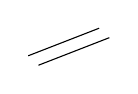
\begin{tikzpicture}[x=1cm,y=1cm]
\draw (0,0)--(0.9,0.35);
\draw (0.13,-0.12)--(1.03,0.23);
\end{tikzpicture}}

A datum $(X_i^*)_{i\in I}$ satisfying 1°) and 3°) is equivalent to
$=$ : \unsure{of a|a} \uline{local\textsuperscript{ly} finite} and \uline{open} equivalence relation
\deleted{\unsure{such that the classes are|such that the closed sets are}}
and $I$ is the quotient space (with the specialization \inserted{pre}order
relation), \deleted{\illegible{3}} the set $I$ is \uline{ordered} if and only if
\[
(\forall i,j\quad\overline{X_i^*}=\overline{X_j^*}\Rightarrow i=j)
\Longleftrightarrow(\text{the }X_i\text{ are locally closed}).
\]

\margin{case $I$ \uline{ordered} $\Updownarrow$}
\uline{Strict} \uline{stratification}

locally finite \inserted{increasing} family $(X_i)_{i\in I}$ of closed sets, such that $\forall j<i$
implies that $X_j$ nowhere dense in $X_i$, and $\forall i,j\in I$,
one has
\[
X_i\cap X_j=\bigcup_{k\in\overline i\cap\overline j}X_k.
\]
\figure{\begin{tikzpicture}\draw (0,0)--(2.4,0);\end{tikzpicture}}

In the framework of tame topology, one must see how
\inserted{for} every partition into locally closed \uline{tame} subsets,
there exists a smallest \inserted{\unsure{strict|\deleted{strict}|\deleted{strict}} tame stratification}
\deleted{partition} \unsure{(formed)} \unsure{those that|those that|such that}
\deleted{\unsure{dominate|generates}} the given partition.

% The following line records the ruled division between the two manuscript halves.
\figure{\begin{tikzpicture}\draw (0,0)--(0,-3);\end{tikzpicture}}
\mspage{4)}
\margin{\diagram{\begin{tikzcd}[x=0.65cm,y=0.65cm,
column sep=0pt,row sep=0pt,ampersand replacement=\&,
execute at end picture={
\node at (0,0) {$\overline{\unsure{J|I}}$};
\node at (1,0) {$\unsure{J|I}$};
\draw (1.65,-0.65)--(1.65,0.8);
\node at (2.6,0) {$y<x$};
\node at (2.18,1.45) {$\unsure{J|\supset}$};
\node at (2.18,0.8) {$\unsure{\Downarrow|\notin}$};
\node at (3.03,0.8) {$\in J$};
\draw (1.94,-0.4)--(2.09,-0.4);
\node at (5.2,0) {$x\in J$};
}]
{}
\end{tikzcd}}}

$(X_i^*)_{i\in I}$ an \inserted{indexed partition} \deleted{family}
(locally finite \inserted{of $X$} \deleted{\unsure{of disjoint subsets of $X$, with union $X$, i.e. an $X\xrightarrow{\varphi}I$}}). Equivalent conditions.

a) $\forall i\in I$, \deleted{\unsure{the $X_i^*\ne\phi$ (i.e. $\varphi$ surjective, i.e. a partition), and}}
$\overline{X_i^*}$ is saturated \deleted{\unsure{for the $X_i^*$ is locally closed|for the $X_i^*$ and locally closed}}

b) $\exists\leq$ a \deleted{relation} \inserted{pre}order on $I$, such that one has $\forall i\in I$
\[
\overline{X_i^*}=\bigcup_{j\in\overline i}X_j^*
\]
(\unsure{this|\deleted{this}} \deleted{relation} preorder is unique, \ldots
\[
i\leq j\Longleftrightarrow\overline{X_i^*}\subset\overline{X_j^*}\unsure{\rbrace|)}
\quad(\Longleftrightarrow X_i^*\subset\overline{X_j^*})
\]
c) The quotient topology of $I$ is such that $\varphi:X\longrightarrow I$ is open,
i.e. $\forall U\in\operatorname{Ouv}(X)$, the saturation is open

Under these conditions, the quotient topology of $I$ is the one
associated with \deleted{\unsure{its order relation|the order relation}} preorder, which is also
the specialization relation for this topology.
For $I$ to be ordered, it is necessary and sufficient that the
$X_i^*$ be local\textsuperscript{ly}\unsure{.} closed. One then says that the partition is
\uline{stratifying} \unsure{(i.e. the $X_i^*$ saturated)|\deleted{(i.e. the $X_i^*$ saturated)}}.
\inserted{\unsure{the|\deleted{the}|\illegible{1}} locally finite, locally closed pieces, open equivalence relation}

We have a 1--1 \uuline{correspondence} between the
\inserted{stratifying} partitions of $X$ of this form, i.e. the locally
finite and open equivalence relations, \inserted{on $X$, with locally closed fibers}, and the set of families (up to isomorphism)
$(X_i)_{i\in I}$ indexed by an \uline{ordered}
\inserted{\uline{locally finite}} index set $I$,
which are such that 1°) \uline{\unsure{increasing|increasing}} \unsure{family|families} of
\inserted{\uline{closed}} \deleted{\unsure{increasing}} subsets of $X$, \deleted{\unsure{and}} \uline{covering} $X$, and 2°) $\forall i,j\in I$
\[
X_i\cap X_j=\bigcup_{k\in\overline i\cap\overline j}X_k
\]
\inserted{4°) \deleted{$\unsure{X_k|X_\alpha}$} $\forall i,j\in I$, $j<i$
$\Longrightarrow$ \deleted{\illegible{1}} $X_j$ \uline{nowhere dense} \uline{in} $X_i$
\unsure{($\forall i$, i.e. $\unsure{X_i^*|\overline{X_i^*}}=X_i$)|(i.e. $\overline{X_i^*}=X_i$)}}
\inserted{3°) $\forall i$, $\underset{\substack{\Vert\,\mathrm{definition}\\X_i\setminus\bigcup_{j<i}X_j}}{X_i^*}\ne\phi$}

\margin{\uline{NB} Assuming 1°, 2°, 4°, 3° is equivalent to
the weaker condition
3 bis) $(\forall i\in I)$ $\unsure{X_i|X}\ne\phi$.}

Assuming 1°) and 2°), setting $X_i^*=X_i\setminus\bigcup_{j<i}X_j^*$,
the $X_i^*$ form a \inserted{locally finite} \unsure{p.|ps.} partition of $X$ into
locally closed sets; this satisfies the conditions
of a \uline{strict} \uline{stratifying} \uline{partition}, \inserted{for the order given to $I$} if and only if
one has 3°) and 4°).

\uline{Stratification} : Conditions \unsure{1°) and 2°)|2°) and 1°)}. \uline{Strict stratification} : ``faithful'' (i.e.
3°) and density condition (4°) : \unsure{Stratifying|Stratifying} partitions $\unsure{\Longleftarrow|\Longleftrightarrow}$ \unsure{strict|strict} stratification
\margin{3}
